
\documentclass[]{article}

\title{TEOREMA DEL LÍMITE CENTRAL}

\date{}
\usepackage{braket}
\usepackage{bbold}
\usepackage{amsmath,amsfonts,amssymb,amsthm,booktabs}
\usepackage[margin=1.0in]{geometry}
\usepackage{graphicx}
\usepackage{chngcntr}
\usepackage{floatrow}
\usepackage{chngcntr}
\usepackage{hyperref}
\usepackage[spanish]{babel}
\usepackage[svgnames]{xcolor}
\usepackage{commath}
\usepackage{floatrow}
\floatsetup[table]{capposition=top}
\DeclareRobustCommand{\bbone}{\text{\usefont{U}{bbold}{m}{n}1}}

\DeclareMathOperator{\EX}{\mathbb{E}}% expected val
\renewcommand{\spanishtablename}{Cuadro}
\usepackage{listings}
\usepackage[%
    font={small,sf},
    labelfont=bf,
    format=hang,    
    format=plain,
    margin=0pt,
    width=0.8\textwidth,
]{caption}
\usepackage[list=true]{subcaption}
\lstset{language=R,
    basicstyle=\small\ttfamily,
    stringstyle=\color{DarkGreen},
    otherkeywords={0,1,2,3,4,5,6,7,8,9},
    morekeywords={TRUE,FALSE},
    deletekeywords={data,frame,length,as,character},
    keywordstyle=\color{blue},
    commentstyle=\color{DarkGreen},
}

\counterwithin{figure}{section}
\renewcommand*{\figureautorefname}{Figura}


\usepackage[backend=biber]{biblatex}
\addbibresource{ref.bib}

\begin{document}
	\maketitle
	\begin{center}


\centerline{\textbf{TAREA 14} } 
\textbf{ }

\centerline{Alumno: } 
\centerline{Joaquín Arturo Velarde Moreno}


	\end{center}
	

\section{Introducción}

El objetivo de esta tarea es explicar como se puede aplicar el teorema de limite central, para analizar una población de la que no se conoce ni su media ni su varianza, las cuales queremos aproximar, puesto que nos interesa hacer inferencia sobre esta población en general, siendo estos dos parámetros los mas importantes para realizar inferencia. Estos conceptos de probabilidad son introducidos en el material del curso de modelos probabilistas aplicados\cite{MaterialClase} y ademas con el uso de R poder comprobar numéricamente sus propiedades\cite{rproject}, este documento se encuentra alojado en el repositorio\cite{repositorio} como recurso libre.

\section{Teorema del límite central}
Una muestra de tamaño \textit{n} de una población por definición tiene una media:
\[ p = \frac{X_{1} + X_{2} +...X_{n}}{n}.\]
Donde:
\begin{itemize}
	\item $n$ es el numero de elementos de la muestra,
	\item $X_{n}$ cada elemento de la muestra,
	\item $p$ es la media muestral.
\end{itemize}
Y una varianza muestral:
\[ \sigma_{p}^{2} = \frac{1}{n}\sum_{i=1}^{n}(X_ {i} - p)^{2}.\]
Donde:
\begin{itemize}
	\item $n$ es el numero de elementos de la muestra,
	\item $X_{i}$ cada elemento de la muestra,
	\item $\sigma_{p}^{2}$ es varianza.
\end{itemize}
Ademas la desviación estándar de la muestra esta relacionada con la desviación típica de la distribución de probabilidad real de la población.
\[ \sigma_{p} = \frac{\sigma}{\sqrt{n}}.\]
Donde:
\begin{itemize}
	\item $\sigma$ es la desviación estándar de la población,
	\item $n$ tamaño de la muestra,
	\item $\sigma_{p}$ es la desviación estándar de la muestra.
\end{itemize}
El teorema central del limite dice que, bajo condiciones más bien generales, las medias obtenidas de muestras aleatorias de una población tienden a tener una distribución que se aproxima a la normal.\\
Teorema: Tenemos por $f(x)$ una densidad con $\mu$ y varianza finita $\sigma^{2}$ y sea $p$ la media de una muestra aleatoria de tamaño $n$ de $f(x)$ definimos la variable aleatoria $Y$ por la distribución de $Y$ se aproxima a la normal de media cero y varianza uno cuando $n$ crece indefinidamente.
\[ Y_{p} = \frac{p_{n} - \mu}{\sigma}\sqrt{n}.\]

Podemos observar este comportamiento en R \cite{rproject}, supongamos que tenemos una distribución exponencial con $n$ datos(\autoref{fig:casoexp}).
  \begin{lstlisting}
  n      <- 500
  vector <- rexp(n,2)
   \end{lstlisting}
\begin{figure}[hbt!]
\centering{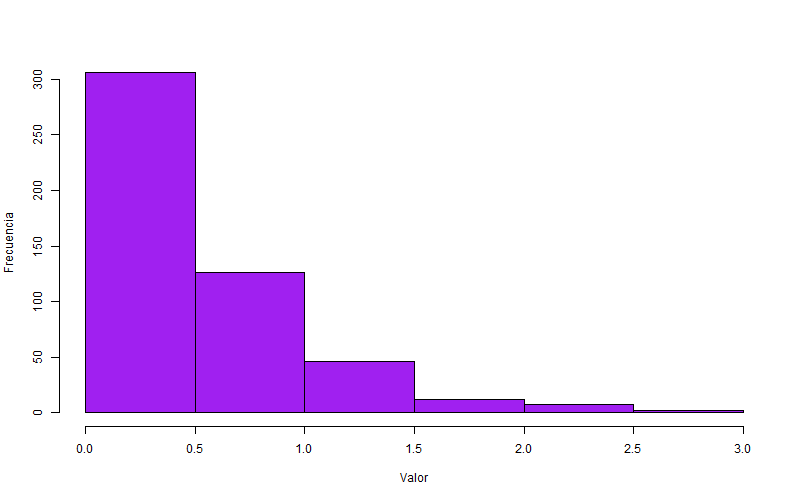
\includegraphics[width=0.8\textwidth]{Figuras/exp.png}}%
\hfill
\caption{Distribución exponencial de $n$ muestras.}

\label{fig:casoexp}
\end{figure}
Ahora obtendremos una muestra aleatoria de elementos de esta y sacaremos su media muestral un numero $n$ de veces.
  \begin{lstlisting}
  n           <- 500
  vector      <- rexp(n,2)
  nmuestral   <- 50
  for(i in 1:n)
  {
    sample    <- sample(vector, nmuestral)
    medias    <- c(medias, sum(sample)/nmuestral)
  }
   \end{lstlisting}
Si observamos la distribución de las medias obtenidas su distribución se aproximara cada vez mas a una normal (\autoref{fig:casos}).

\begin{figure}[hbt!]
\centering
\subcaptionbox{Distribución del promedio de una muestra de 2 elementos aleatorios.}{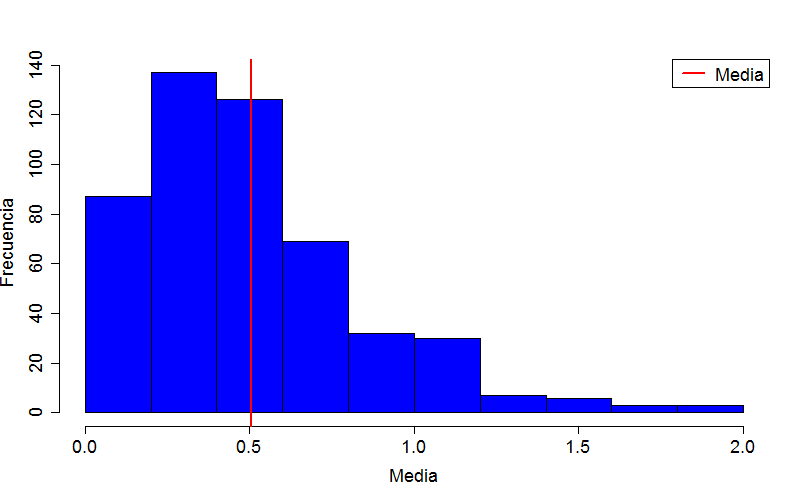
\includegraphics[width=0.5\textwidth]{Figuras/medias_2.png}}%
\hfill
\subcaptionbox{Distribución del promedio de una muestra de 5 elementos aleatorios.}{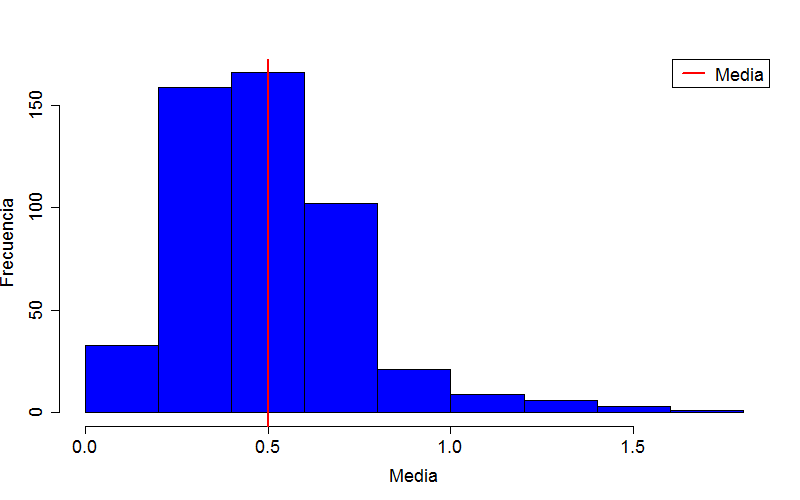
\includegraphics[width=0.5\textwidth]{Figuras/medias_5.png}}%
\hfill
\subcaptionbox{Distribución del promedio de una muestra de 10 elementos aleatorios.}{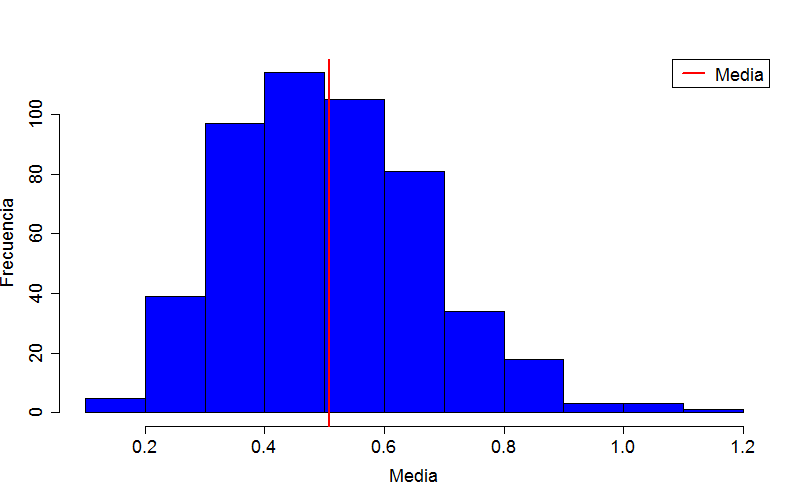
\includegraphics[width=0.5\textwidth]{Figuras/medias_10.png}}%
\hfill
\subcaptionbox{Distribución del promedio de una muestra de 50 elementos aleatorios.}{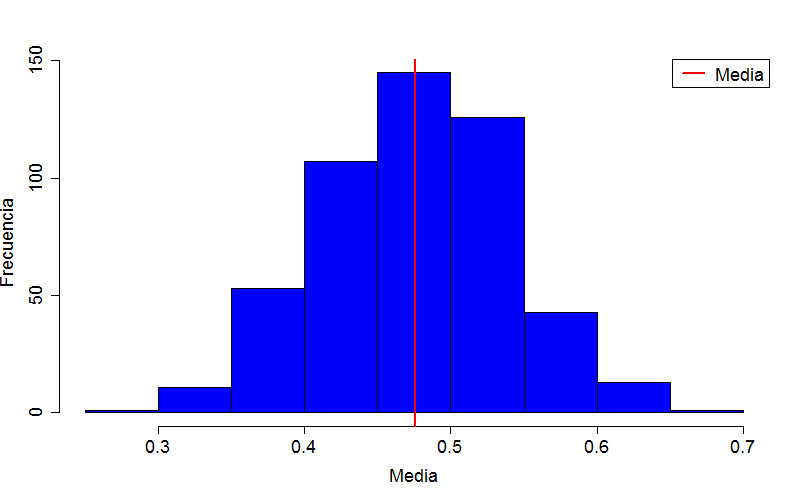
\includegraphics[width=0.5\textwidth]{Figuras/medias_50.png}}% 
\hfill
\caption{Distribuciones de promedio en las muestras obtenidas al ir aumentando el número de muestras.}

\label{fig:casos}
\end{figure}   
\hfill
\section{Aplicación Pizzería}
Un local de pizzas que opera en la Ciudad de México tarda una media de 25 minutos en llevar una pizza,
con una desviación típica de 7 minutos. Supongamos que durante el día de hoy han repartido 150
pizzas.
\begin{itemize}
	\item ¿Cuál es la probabilidad de que la media de los tiempos de entrega de hoy esté entre 20 y 25 minutos?.
\end{itemize}
Consideremos la variable X como tiempo de entrega, 
y sabemos que su media es 25 minutos y su
desviación típica, 5. Pero en general esta variable no sigue una distribución normal.
Durante el día de hoy se han entregado n = 150 paquetes. Es decir, tenemos una muestra $X_{1}, X_{2}, ..., X_{n}$ de nuestra
variable.
Por el teorema del límite central sabemos que la media muestral se comporta como una normal de
esperanza 25 y desviación típica:
$\frac{7}{\sqrt{150}} = 0.571.$

Con estos datos podemos usar la  aproximación a la normal con nuestra variable $p$ para calcular la probabilidad buscada de la siguiente manera:
\[ P(20 \leq p \leq 25) = P(\frac{20-25}{0.571} \leq \frac{p-25}{0.571} \leq \frac{25-25}{0.571}).\]
Que es igual a la siguiente probabilidad:
\[ P(\frac{20-25}{0.572} \leq Y \leq P(\frac{25-25}{0.572}) = P(-8.74 \leq Y \leq 0) = P(Y \leq 0) - P(Y \leq -8.74) = 0.5 - 0.\]

\printbibliography[title={Referencias}]
\end{document}
